% kernel.h — lowering & backend flow diagram (TikZ).
% atom IR -> atom dialect -> gpu.module -> NVVM/ROCDL split -> thin runtime.
% Mirrors the report's TikZ aesthetic (accent RGB{0,60,120}, rounded boxes,
% Stealth arrows). Rendered to a cropped PNG via pdflatex + pdftoppm + trim.
\documentclass[10pt]{article}
\usepackage[T1]{fontenc}
\usepackage[utf8]{inputenc}
\usepackage[margin=0cm]{geometry}
\pagestyle{empty}
\usepackage{xcolor}
\definecolor{accent}{RGB}{0,60,120}
\definecolor{codebg}{RGB}{248,248,248}
\usepackage{tikz}
\usetikzlibrary{arrows.meta,positioning}

\begin{document}
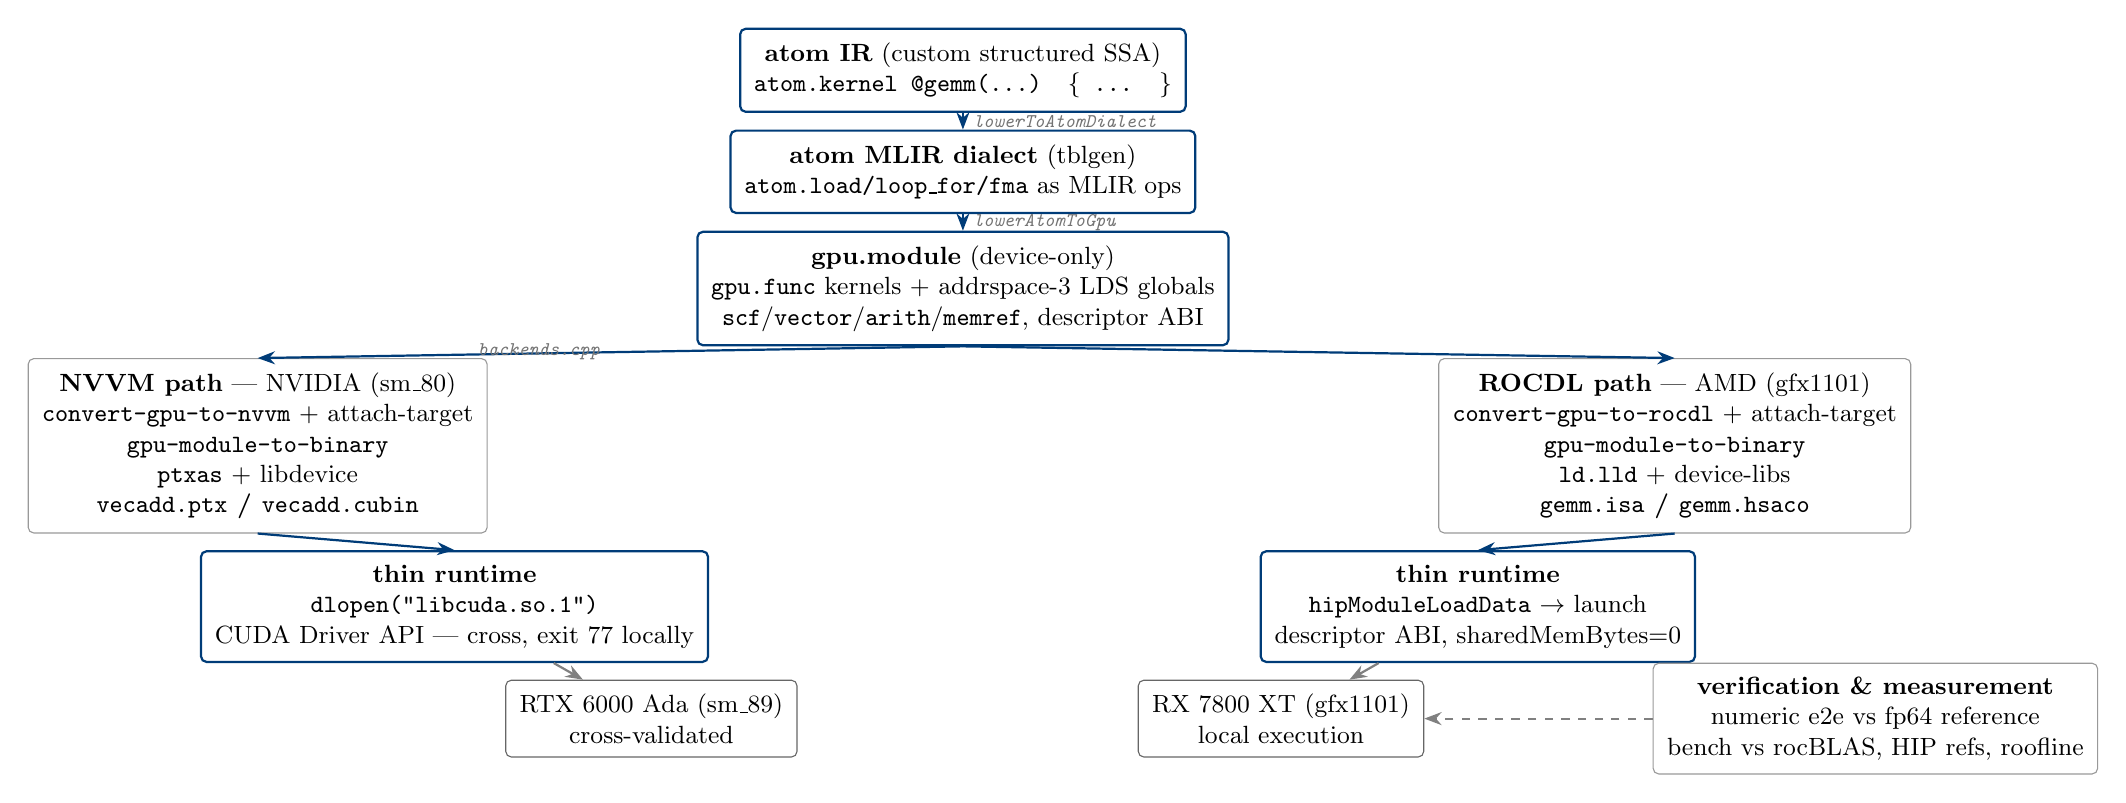
\begin{tikzpicture}[
  node distance=6pt,
  box/.style={draw, rounded corners=2pt, align=center, inner sep=5pt,
              fill=white, font=\small},
  stage/.style={box, draw=accent, thick},
  side/.style={box, draw=black!40, minimum width=5.2cm},
  runtime/.style={box, draw=accent, thick},
  arrow/.style={-{Stealth[length=2.2mm]}, thick, draw=accent},
  srrow/.style={-{Stealth[length=2.2mm]}, thick, draw=black!50},
  lbl/.style={font=\scriptsize\itshape, text=black!55},
]

  % ---- front end: lowering chain ----
  \node[stage] (atomir) {\textbf{atom IR} (custom structured SSA)\\%
    \texttt{atom.kernel @gemm(...) \{ ... \}}};
  \node[stage, below=of atomir] (dialect) {\textbf{atom MLIR dialect} (tblgen)\\%
    \texttt{atom.load/loop\_for/fma} as MLIR ops};
  \node[stage, below=of dialect] (gpumod) {\textbf{gpu.module} (device-only)\\%
    \texttt{gpu.func} kernels + addrspace-3 LDS globals\\%
    \texttt{scf}/\texttt{vector}/\texttt{arith}/\texttt{memref}, descriptor ABI};

  \draw[arrow] (atomir) -- node[lbl, right] {\texttt{lowerToAtomDialect}} (dialect);
  \draw[arrow] (dialect) -- node[lbl, right] {\texttt{lowerAtomToGpu}} (gpumod);

  % ---- vendor split ----
  \node[side, below left=of gpumod, xshift=-2.5cm] (nvvm) {%
    \textbf{NVVM path} — NVIDIA (sm\_80)\\%
    \texttt{convert-gpu-to-nvvm} + attach-target\\%
    \texttt{gpu-module-to-binary}\\%
    \texttt{ptxas} + libdevice\\%
    \textbf{\texttt{vecadd.ptx} / \texttt{vecadd.cubin}}};
  \node[side, below right=of gpumod, xshift=2.5cm] (rocdl) {%
    \textbf{ROCDL path} — AMD (gfx1101)\\%
    \texttt{convert-gpu-to-rocdl} + attach-target\\%
    \texttt{gpu-module-to-binary}\\%
    \texttt{ld.lld} + device-libs\\%
    \textbf{\texttt{gemm.isa} / \texttt{gemm.hsaco}}};

  \draw[arrow] (gpumod.south) -- (nvvm.north) node[midway, lbl, left] {\texttt{backends.cpp}};
  \draw[arrow] (gpumod.south) -- (rocdl.north);

  % ---- runtime ----
  \node[runtime, below=of nvvm, xshift=2.5cm] (rtcuda) {%
    \textbf{thin runtime}\\%
    \texttt{dlopen("libcuda.so.1")}\\%
    CUDA Driver API — cross, exit 77 locally};
  \node[runtime, below=of rocdl, xshift=-2.5cm] (rthip) {%
    \textbf{thin runtime}\\%
    \texttt{hipModuleLoadData} $\to$ launch\\%
    descriptor ABI, sharedMemBytes=0};

  \draw[arrow] (nvvm.south) -- (rtcuda.north);
  \draw[arrow] (rocdl.south) -- (rthip.north);

  % ---- GPU ----
  \node[box, below=of rtcuda, xshift=2.5cm, draw=black!60] (gpunv) {%
    RTX 6000 Ada (sm\_89)\\cross-validated};
  \node[box, below=of rthip, xshift=-2.5cm, draw=black!60] (gpuamd) {%
    RX 7800 XT (gfx1101)\\local execution};
  \draw[srrow] (rtcuda) -- (gpunv);
  \draw[srrow] (rthip) -- (gpuamd);

  % ---- verification branch ----
  \node[side, right=4mm of gpuamd, xshift=2.5cm] (verify) {%
    \textbf{verification \& measurement}\\%
    numeric e2e vs fp64 reference\\%
    bench vs rocBLAS, HIP refs, roofline};
  \draw[srrow, dashed] (verify.west) -- (gpuamd.east);
\end{tikzpicture}
\end{document}
